\chapter{HASIL DAN PEMBAHASAN}
\label{chap:hasilpembahasan}

% Ubah bagian-bagian berikut dengan isi dari hasil dan pembahasan

Bab ini akan membahas hasil dan analisa dari desain sistem yang sudah dibuat dan implementasinya. Pengujian terhadap hasil dibagi menjadi beberap bagian.

\section{Pengujian Performa antar \emph{Weight}}
\label{sec:ujiperforma}
Repositori YOLOv5 menyediakan beberapa \emph{checkpoint} atau \emph{weight} yang merupakan hasil training model YOLOv5 dari dataset COCO yang dimanfaatkan sebagai \emph{pretrained model}. Ekspektasi penggunaan pretrained model ini yaitu bobot yang dihasilkan akan memiliki performa yang lebih tinggi daripada melakukan training tanpa pretrained model sama sekali. \emph{COCO Dataset} ini memiliki 80 \emph{class} berbeda. Seperti disebutkan pada \ref{sec:pelabelandataset} yaitu untuk keperluan penelitian ini hanya memerlukan 2 kelas yaitu "no\textunderscore helmet" dan "with\textunderscore helmet". Pada bagian ini akan dipaparkan dan dibandingkan performa antara tiap bobot yang dihasilkan dengan model pretrained dan yang tidak menggunakan pretrained model.

\subsection{Pengujian Performa \emph{Weight} dari Hasil \emph{Pretrain} COCO Dataset}
\label{subsec:ujiperforma_coco}
Beberapa \emph{pretrained model} yang disedikana dari repositori YOLOv5 yaitu YOLOv5n, YOLOV5s, YOLOv5m, YOLOv5l,YOLOv5l, dan YOLOv5x. Selain beberapa model pretrained tersebut juga ada versi untuk ukuran gammbar 1280 yaitu seri YOLOv5n6 hingga YOLOv5l6. Pada penelitian ini hanya menggunakan variasi YOLOv5n hingga YOLOv5l karena variasi YOLOv5x dan versi seri 6 untuk ukuran gambar 1280 membutuhkan waktu yang lebih lama. Perbedaan - perbedaan yang ada pada bobot - bobot pretrained tersebut berasal dari konfigurasi awal dari training pada dataset COCO yang menggunakan YOLOv5, terutama pada paramter "depth\textunderscore multiple" dan "width\textunderscore multiple".
Proses validasi hasil training dilakukan menggunakan dataset Deteksi Helm Keselamatan Kerja yang pembagiannya dijelaskan pada bagian \ref{sec:preprocessing} yang berjumlah 1200 gambar dengan kelas "no\textunderscore helmet" berjumlah 1322 label dan kelas "with\textunderscore helmet" berjumlah 4294 label. Dari semua \emph{weight} yang dihasilkan dari training menggunkana Dataset Helm Keselamatan Kerja lalu dilakukan validasi yang hasilnya dapat dilihat pada Tabel~\ref{tb:pretraincoco}.


\begin{longtable}{|c|c|c|c|c|}
  \caption{Hasil Validasi \emph{Weight} dari Hasil Pretrain}
  \label{tb:pretraincoco}\\
  \hline
  \rowcolor[HTML]{C0C0C0}
  \textbf{\emph{Pretrained Weight}} & \emph{Precision}  & \emph{Recall} & \emph{mAP@.5} & \emph{Inference Time}\\
  \hline
  YOLOv5n                           & 0.92               & 0.878         & 0.922         & 1.9ms              \\
  YOLOv5s                           & 0.927              & 0.882         & 0.929         & 4.1ms              \\
  YOLOv5m                           & 0.923              & 0.892         & 0.933        & 9ms                  \\
  YOLOv5l                           & 0.917              & 0.87          & 0.919         & 13.9ms                \\
  \hline
\end{longtable}

Berdasarkan hasil validasi, tidak ada perbedaan signifikan dari \emph{precision, recall, mAP}. Tetapi perbedaan besar ada pada \emph{inference time}-nya. 

\subsection{Pengujian Performa \emph{Weight} Hasil Train Murni Dataset Deteksi Helm Keselamatan Kerja}
\label{subsec:murnidataset}

Pada bagian ini akan dipaparkan hasil validasi dari \emph{weight} yang dihasilkan dari train tanpa menggunakan \emph{pretrained weight} yang disediakan dari repositori YOLOv5. Untuk proses training, akan digunakan konfigurasi yang serupa dengan konfigurasi yang digunakan pada \emph{weight} yang disediakan repositori YOLOv5.

\begin{longtable}{|c|c|c|c|c|}
  \caption{hasil Validasi \emph{Weight} dari Murni Dataset}
  \label{tb:nopretrain}\\
  \hline
  \rowcolor[HTML]{C0C0C0}
  \textbf{\emph{Configuration}} & \emph{Precision}  & \emph{Recall} & \emph{mAP@.5} & \emph{Inference Time}\\
  \hline
  YOLOv5n                           & 0.918              & 0.85         & 0.909         & 2.4ms                \\
  YOLOv5s                           & 0.927             & 0.865        & 0.919        & 4.1ms               \\
  YOLOv5m                           & 0.939            & 0.862        & 0.924        & 8.7ms                \\
  YOLOv5l                           &                   &             &               &                \\
  \hline
\end{longtable}

Dari \emph{precision, recall, mAP} tidak berbeda jauh dengan yang menggunakan pretrained checkpoint begitu juga dari \emph{inference time} nya.

\section{Pengujian Performa Berdasarkan Jarak}
\label{sec:ujiberdasarkanjarak}

Pada bagian ini akan dipaparkan hasil deteksi pada dataset validasi yang dibagi menjadi beberapa variasi jarak dari kamera. Dataset yang digunakan meliputi 8 foto untuk masing - masing jarak.

\subsection{Pengujian Pada Jarak 1.3 Meter}
\label{subsec:ujijarak1_3meter}



\begin{figure}[ht]
  \centering
  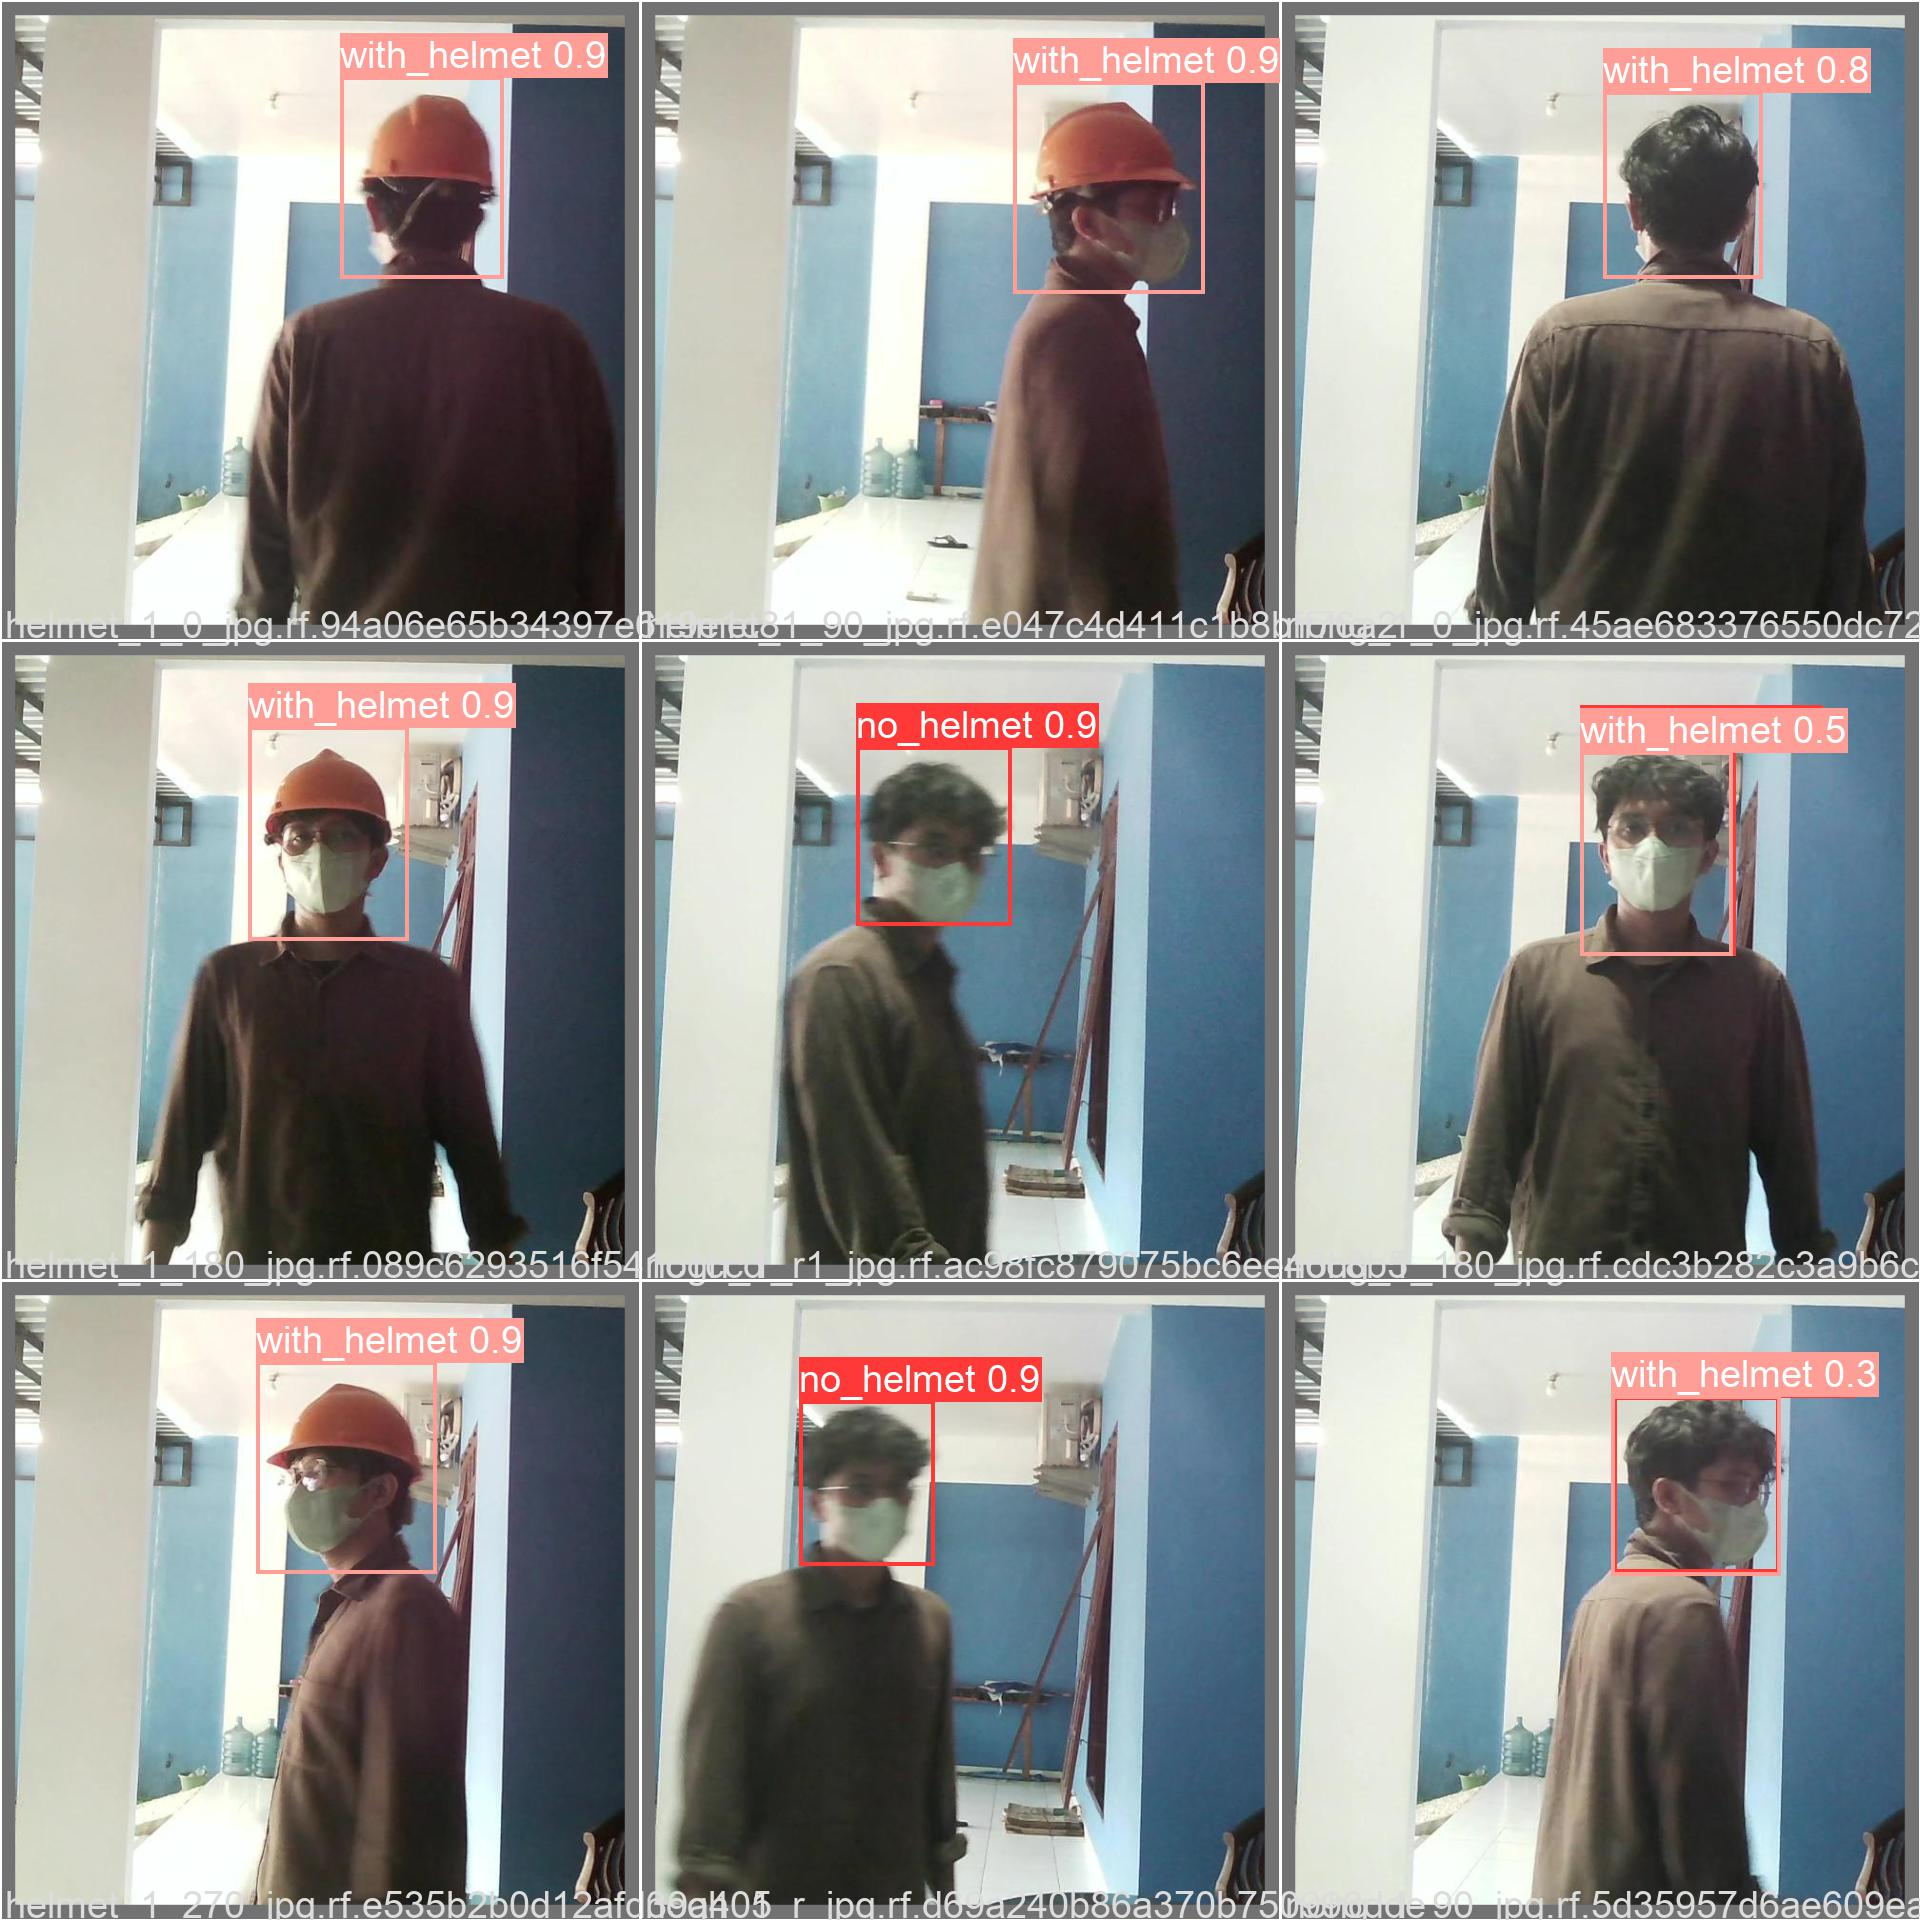
\includegraphics[scale=0.1]{gambar/BerdasarkanJarak/Jarak1_3/val_batch0_pred.jpg}
  \caption{Hasil Prediksi Pada Jarak 1.3 meter}
  % \label{fig:labelbaru}  
\end{figure}

\begin{longtable}{|c|c|c|c|}
  \caption{Konfigurasi Training menggunakan YOLOv5}
  \label{tb:wkwkw}\\
  \hline
  % \rowcolor[HTML]{C0C0C0}
  \textbf{\emph{Class} }                     & \textbf{\emph{Precision}}  & \textbf{\emph{Recall}} & \textbf{\emph{mAP@.5}}\\
  \hline
  all                                                 & 0.998           & 0.8     & 0.995         \\
  no\textunderscore helmet                            & 1               & 0.6       & 0.995          \\
  with\textunderscore helmet                          & 0.996           & 1       & 0.995            \\
  \hline
\end{longtable}

\subsection{Pengujian Pada Jarak 2.6 Meter}

\begin{figure}[ht]
  \centering
  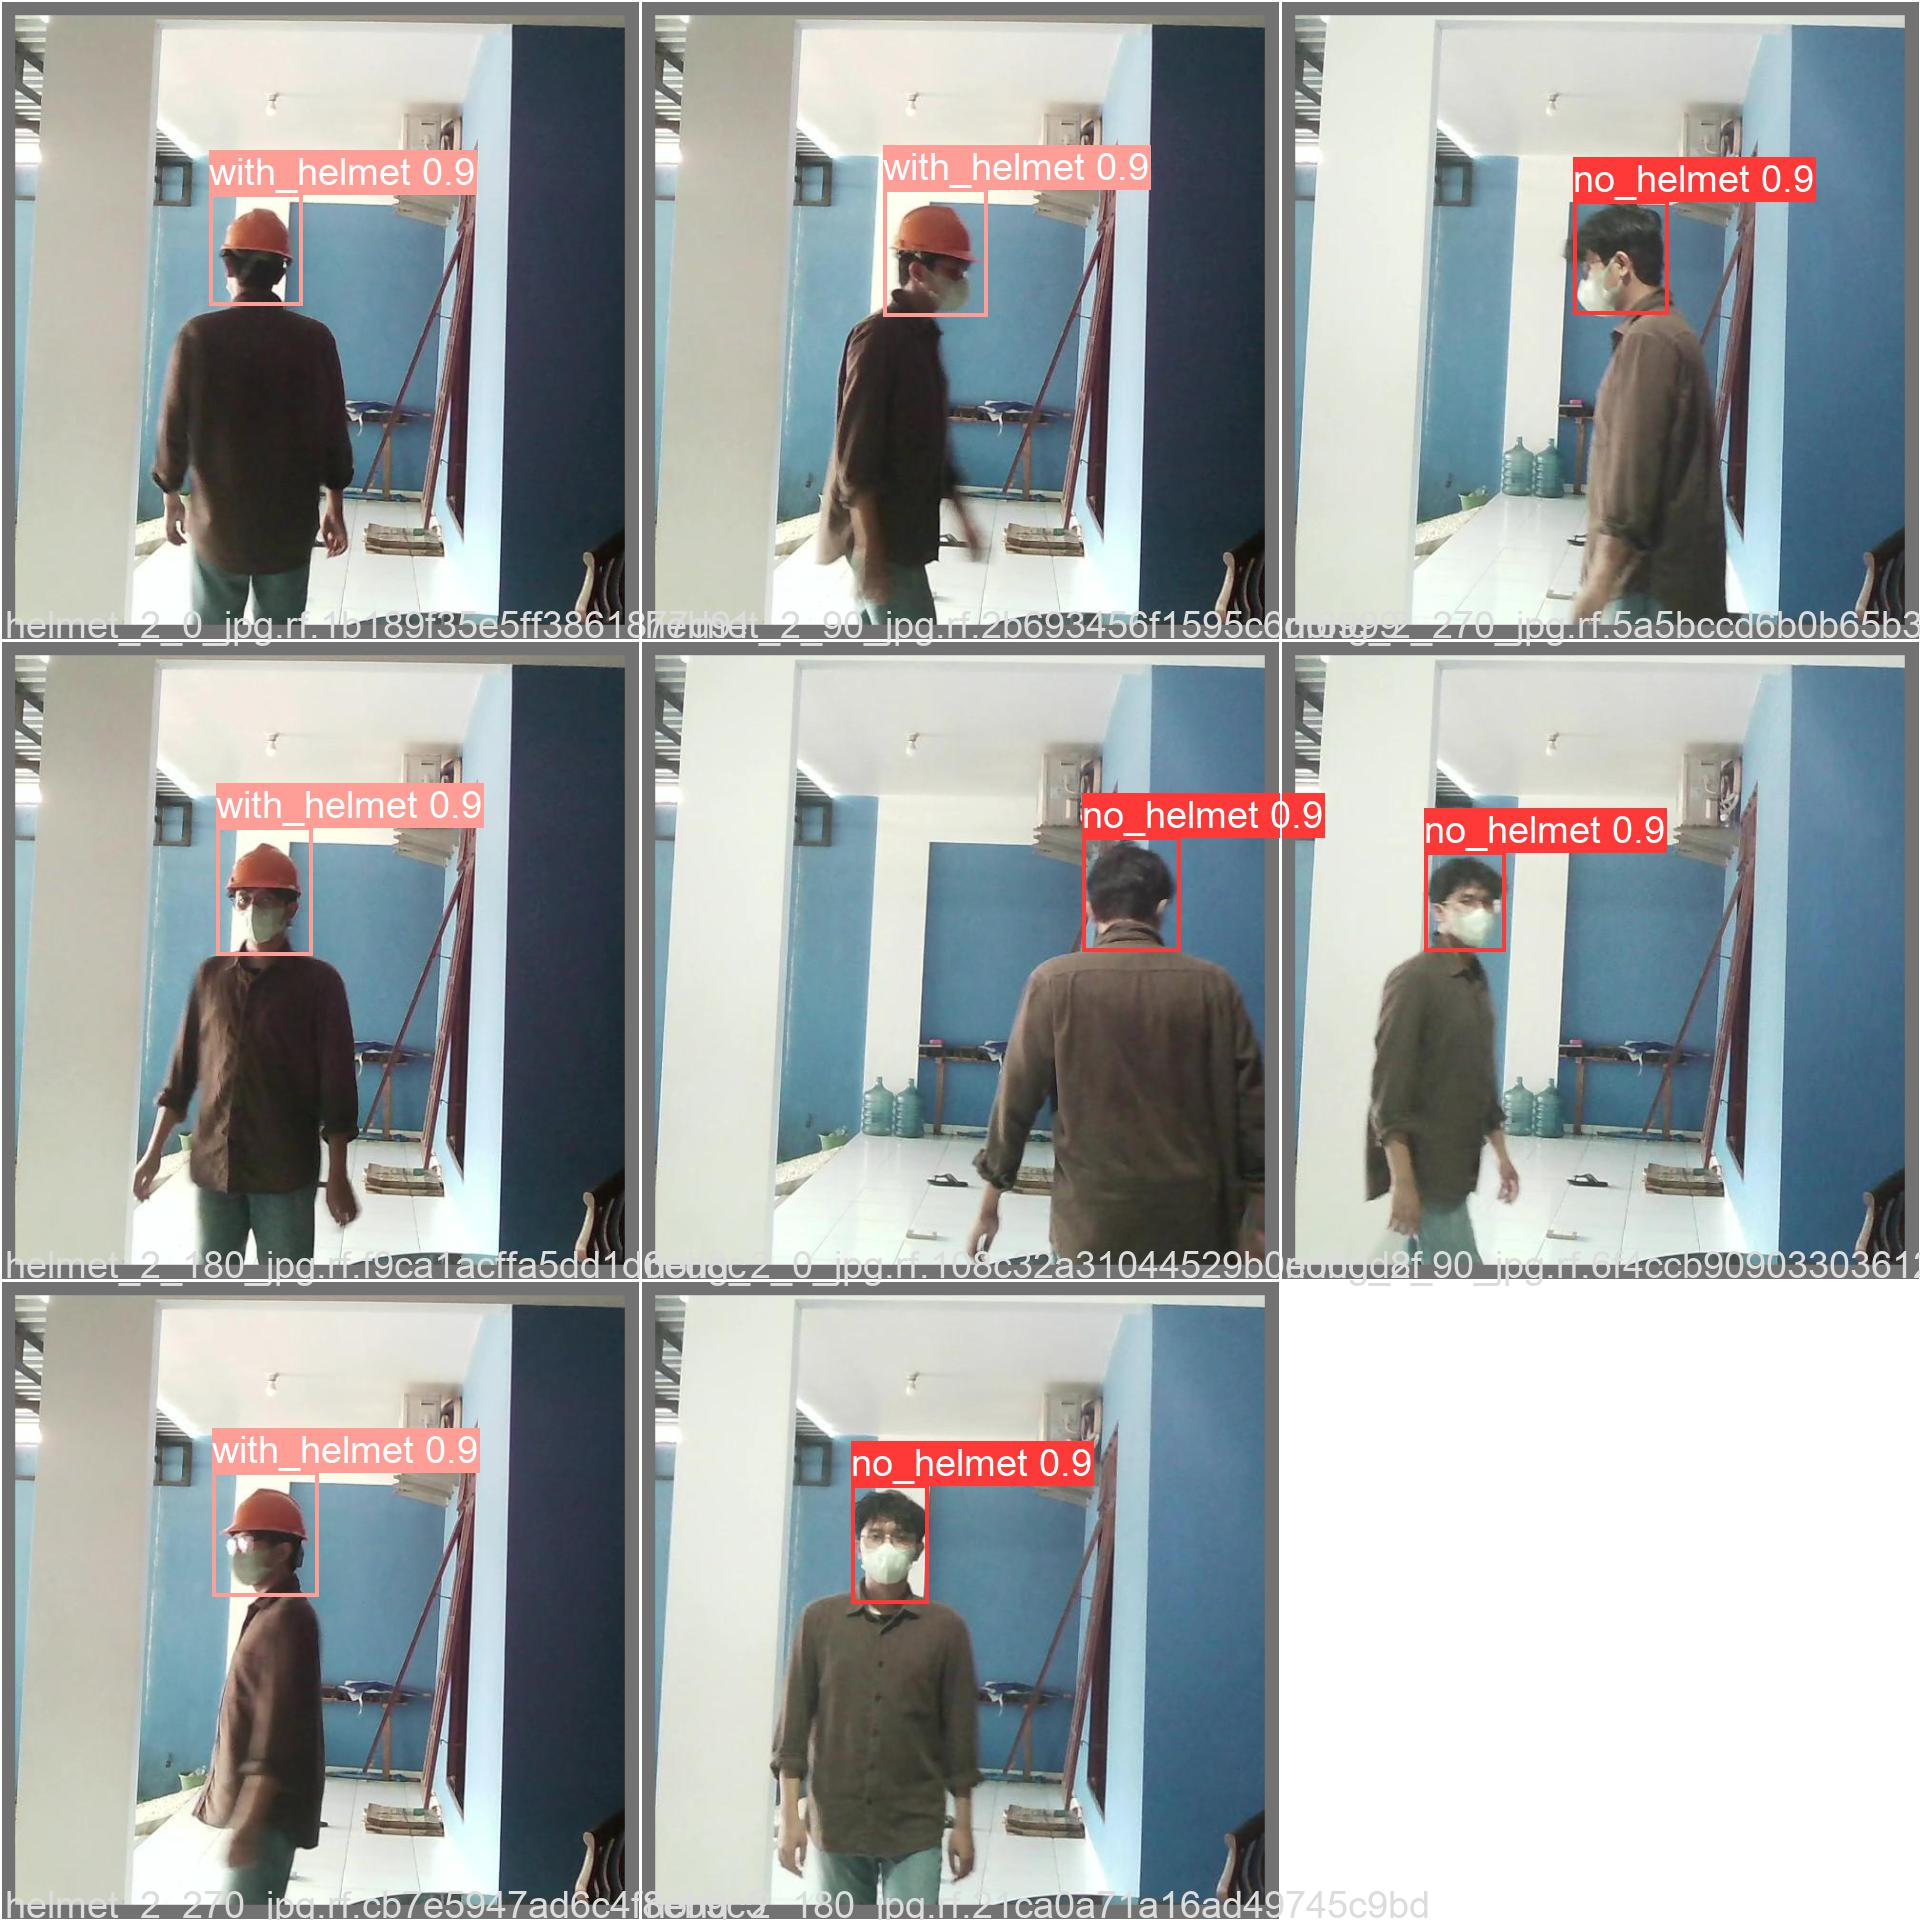
\includegraphics[scale=0.1]{gambar/BerdasarkanJarak/Jarak2_6/val_batch0_pred.jpg}
  \caption{Hasil Prediksi Pada Jarak 2.6 meter}
  % \label{fig:labelbaru}  
\end{figure}

\begin{longtable}{|c|c|c|c|}
  \caption{Konfigurasi Training menggunakan YOLOv5}
  \label{tb:jarak2_6}\\
  \hline
  % \rowcolor[HTML]{C0C0C0}
  \textbf{\emph{Class} }                     & \textbf{\emph{Precision}}  & \textbf{\emph{Recall}} & \textbf{\emph{mAP@.5}}\\
  \hline
  all                                                 & 0.996            & 1        & 0.995         \\
  no\textunderscore helmet                            & 1                & 1        & 0.995          \\
  with\textunderscore helmet                          & 0.992            & 1        & 0.995           \\
  \hline
\end{longtable}

\subsection{Pengujian Pada Jarak 4 Meter}

\begin{figure}[t]
  \centering
  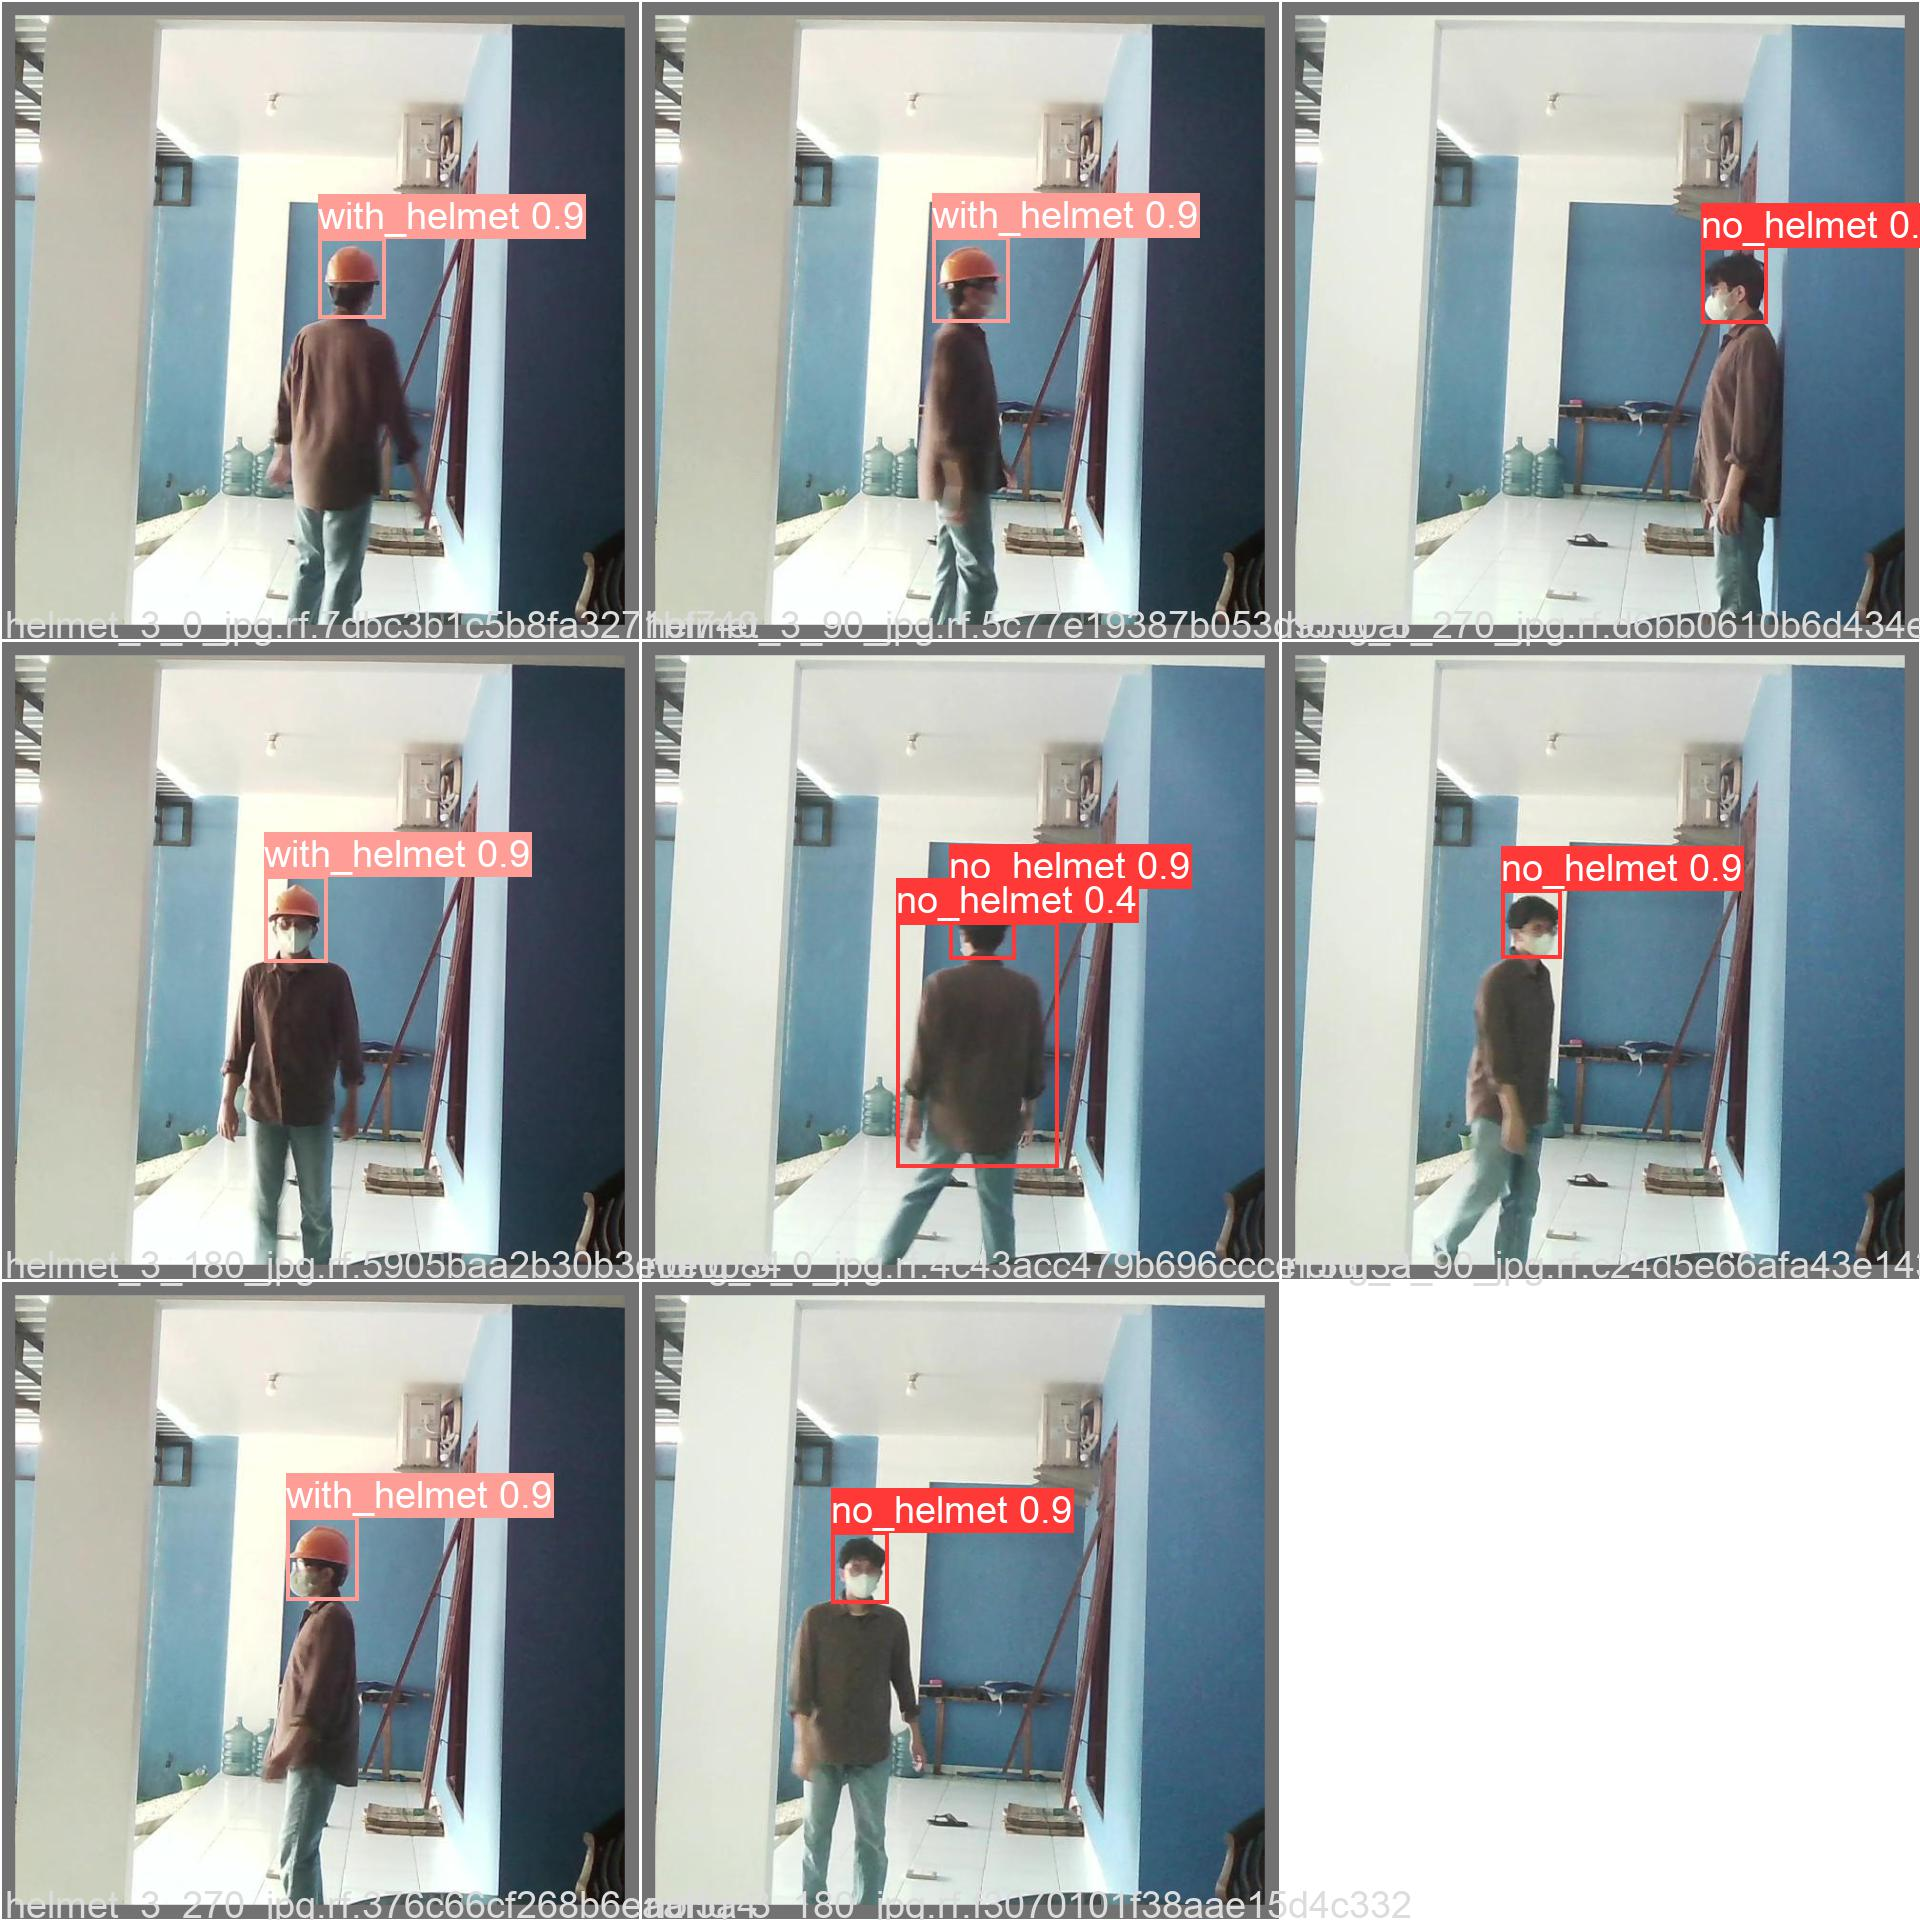
\includegraphics[scale=0.1]{gambar/BerdasarkanJarak/Jarak4/val_batch0_pred.jpg}
  \caption{Hasil Prediksi Pada Jarak 4 meter}
  % \label{fig:labelbaru}  
\end{figure}

\begin{longtable}{|c|c|c|c|}
  \caption{Konfigurasi Training menggunakan YOLOv5}
  \label{tb:jarak4}\\
  \hline
  % \rowcolor[HTML]{C0C0C0}
  \textbf{\emph{Class} }                     & \textbf{\emph{Precision}}  & \textbf{\emph{Recall}} & \textbf{\emph{mAP@.5}}\\
  \hline
  all                                                 & 0.981           & 1        & 0.995         \\
  no\textunderscore helmet                            & 1               & 1        & 0.995          \\
  with\textunderscore helmet                          & 0.963           & 1        & 0.995           \\
  \hline
\end{longtable}

\subsection{Pengujian Pada Jarak 5.3 Meter}

Hasil validasi untuk jarak 5.3 meter masih memiliki tingkat presisi diatas 0.9.

\begin{figure}[ht]
  \centering
  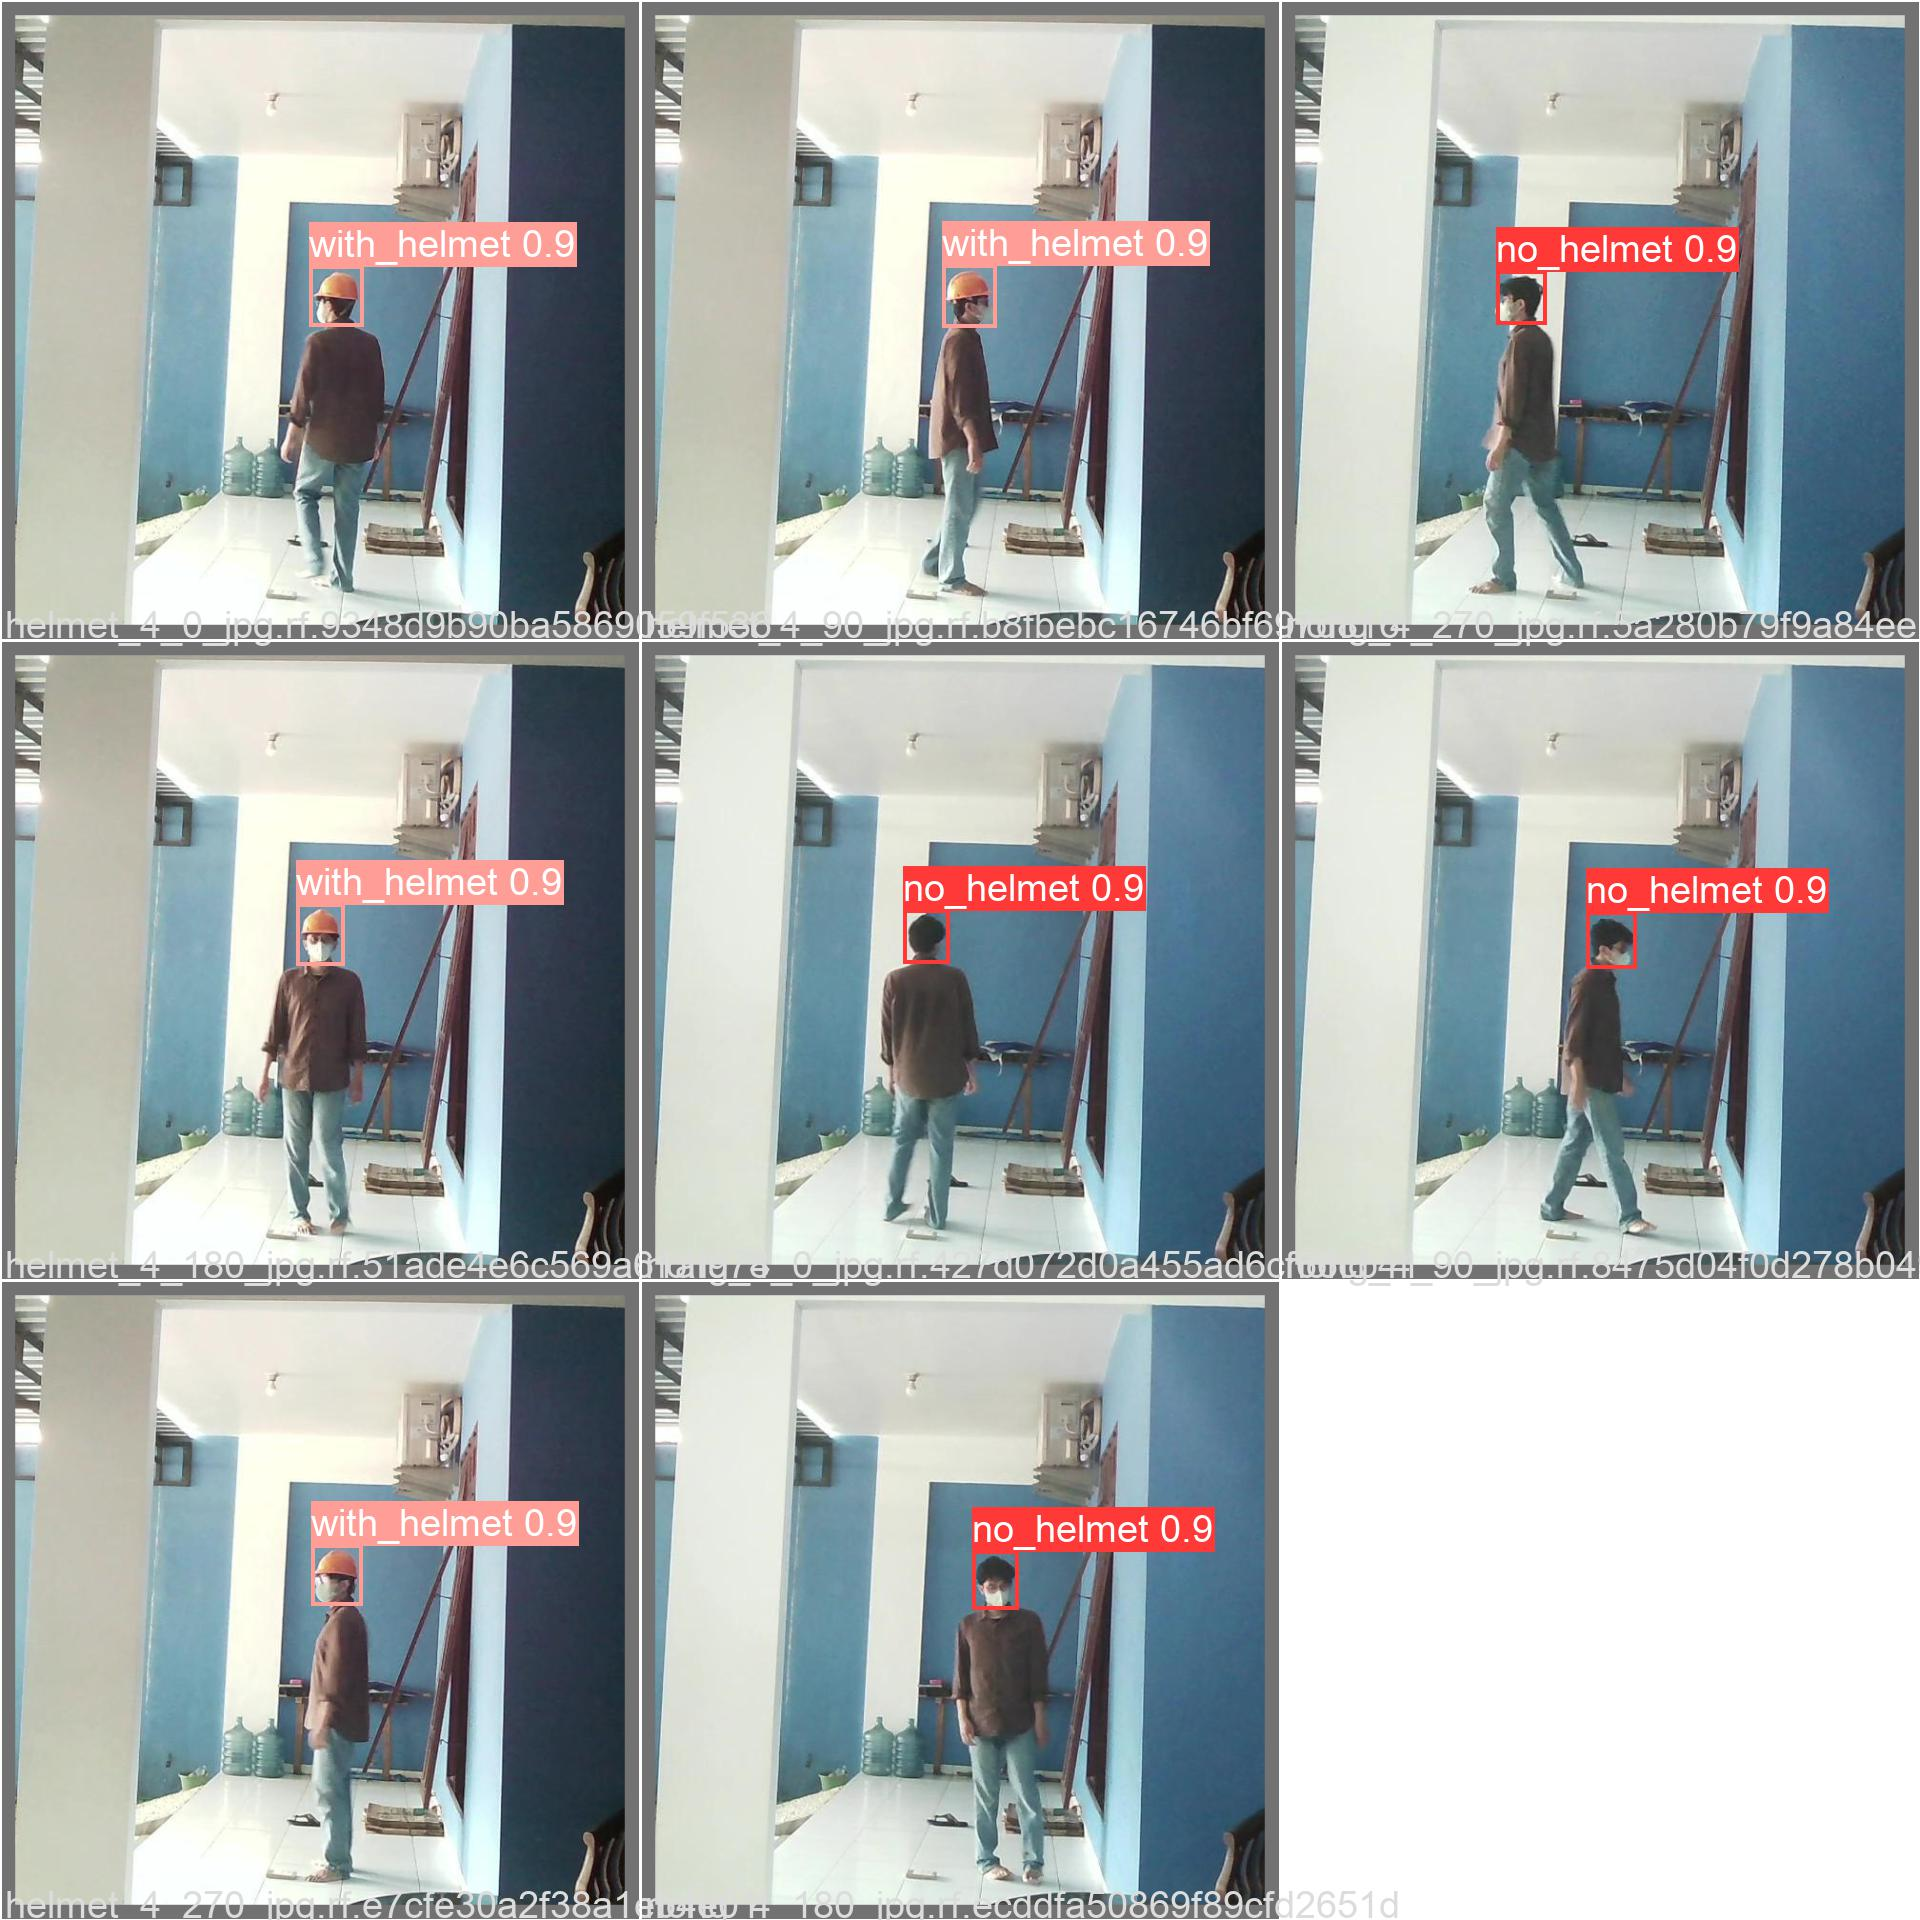
\includegraphics[scale=0.1]{gambar/BerdasarkanJarak/Jarak5_3/val_batch0_pred.jpg}
  \caption{Hasil Prediksi Pada Jarak 5.3 meter}
  % \label{fig:labelbaru}  
\end{figure}

\begin{longtable}{|c|c|c|c|}
  \caption{Konfigurasi Training menggunakan YOLOv5}
  \label{tb:jarak5_3}\\
  \hline
  % \rowcolor[HTML]{C0C0C0}
  \textbf{\emph{Class} }                     & \textbf{\emph{Precision}}  & \textbf{\emph{Recall}} & \textbf{\emph{mAP@.5}}\\
  \hline
  all                                                 & 0.997           & 1        & 0.995         \\
  no\textunderscore helmet                            & 1               & 1        & 0.995          \\
  with\textunderscore helmet                          & 0.995           & 1        & 0.995           \\
  \hline
\end{longtable}

\subsection{Pengujian Pada Jarak 6.7 Meter}

\begin{figure}[ht]
  \centering
  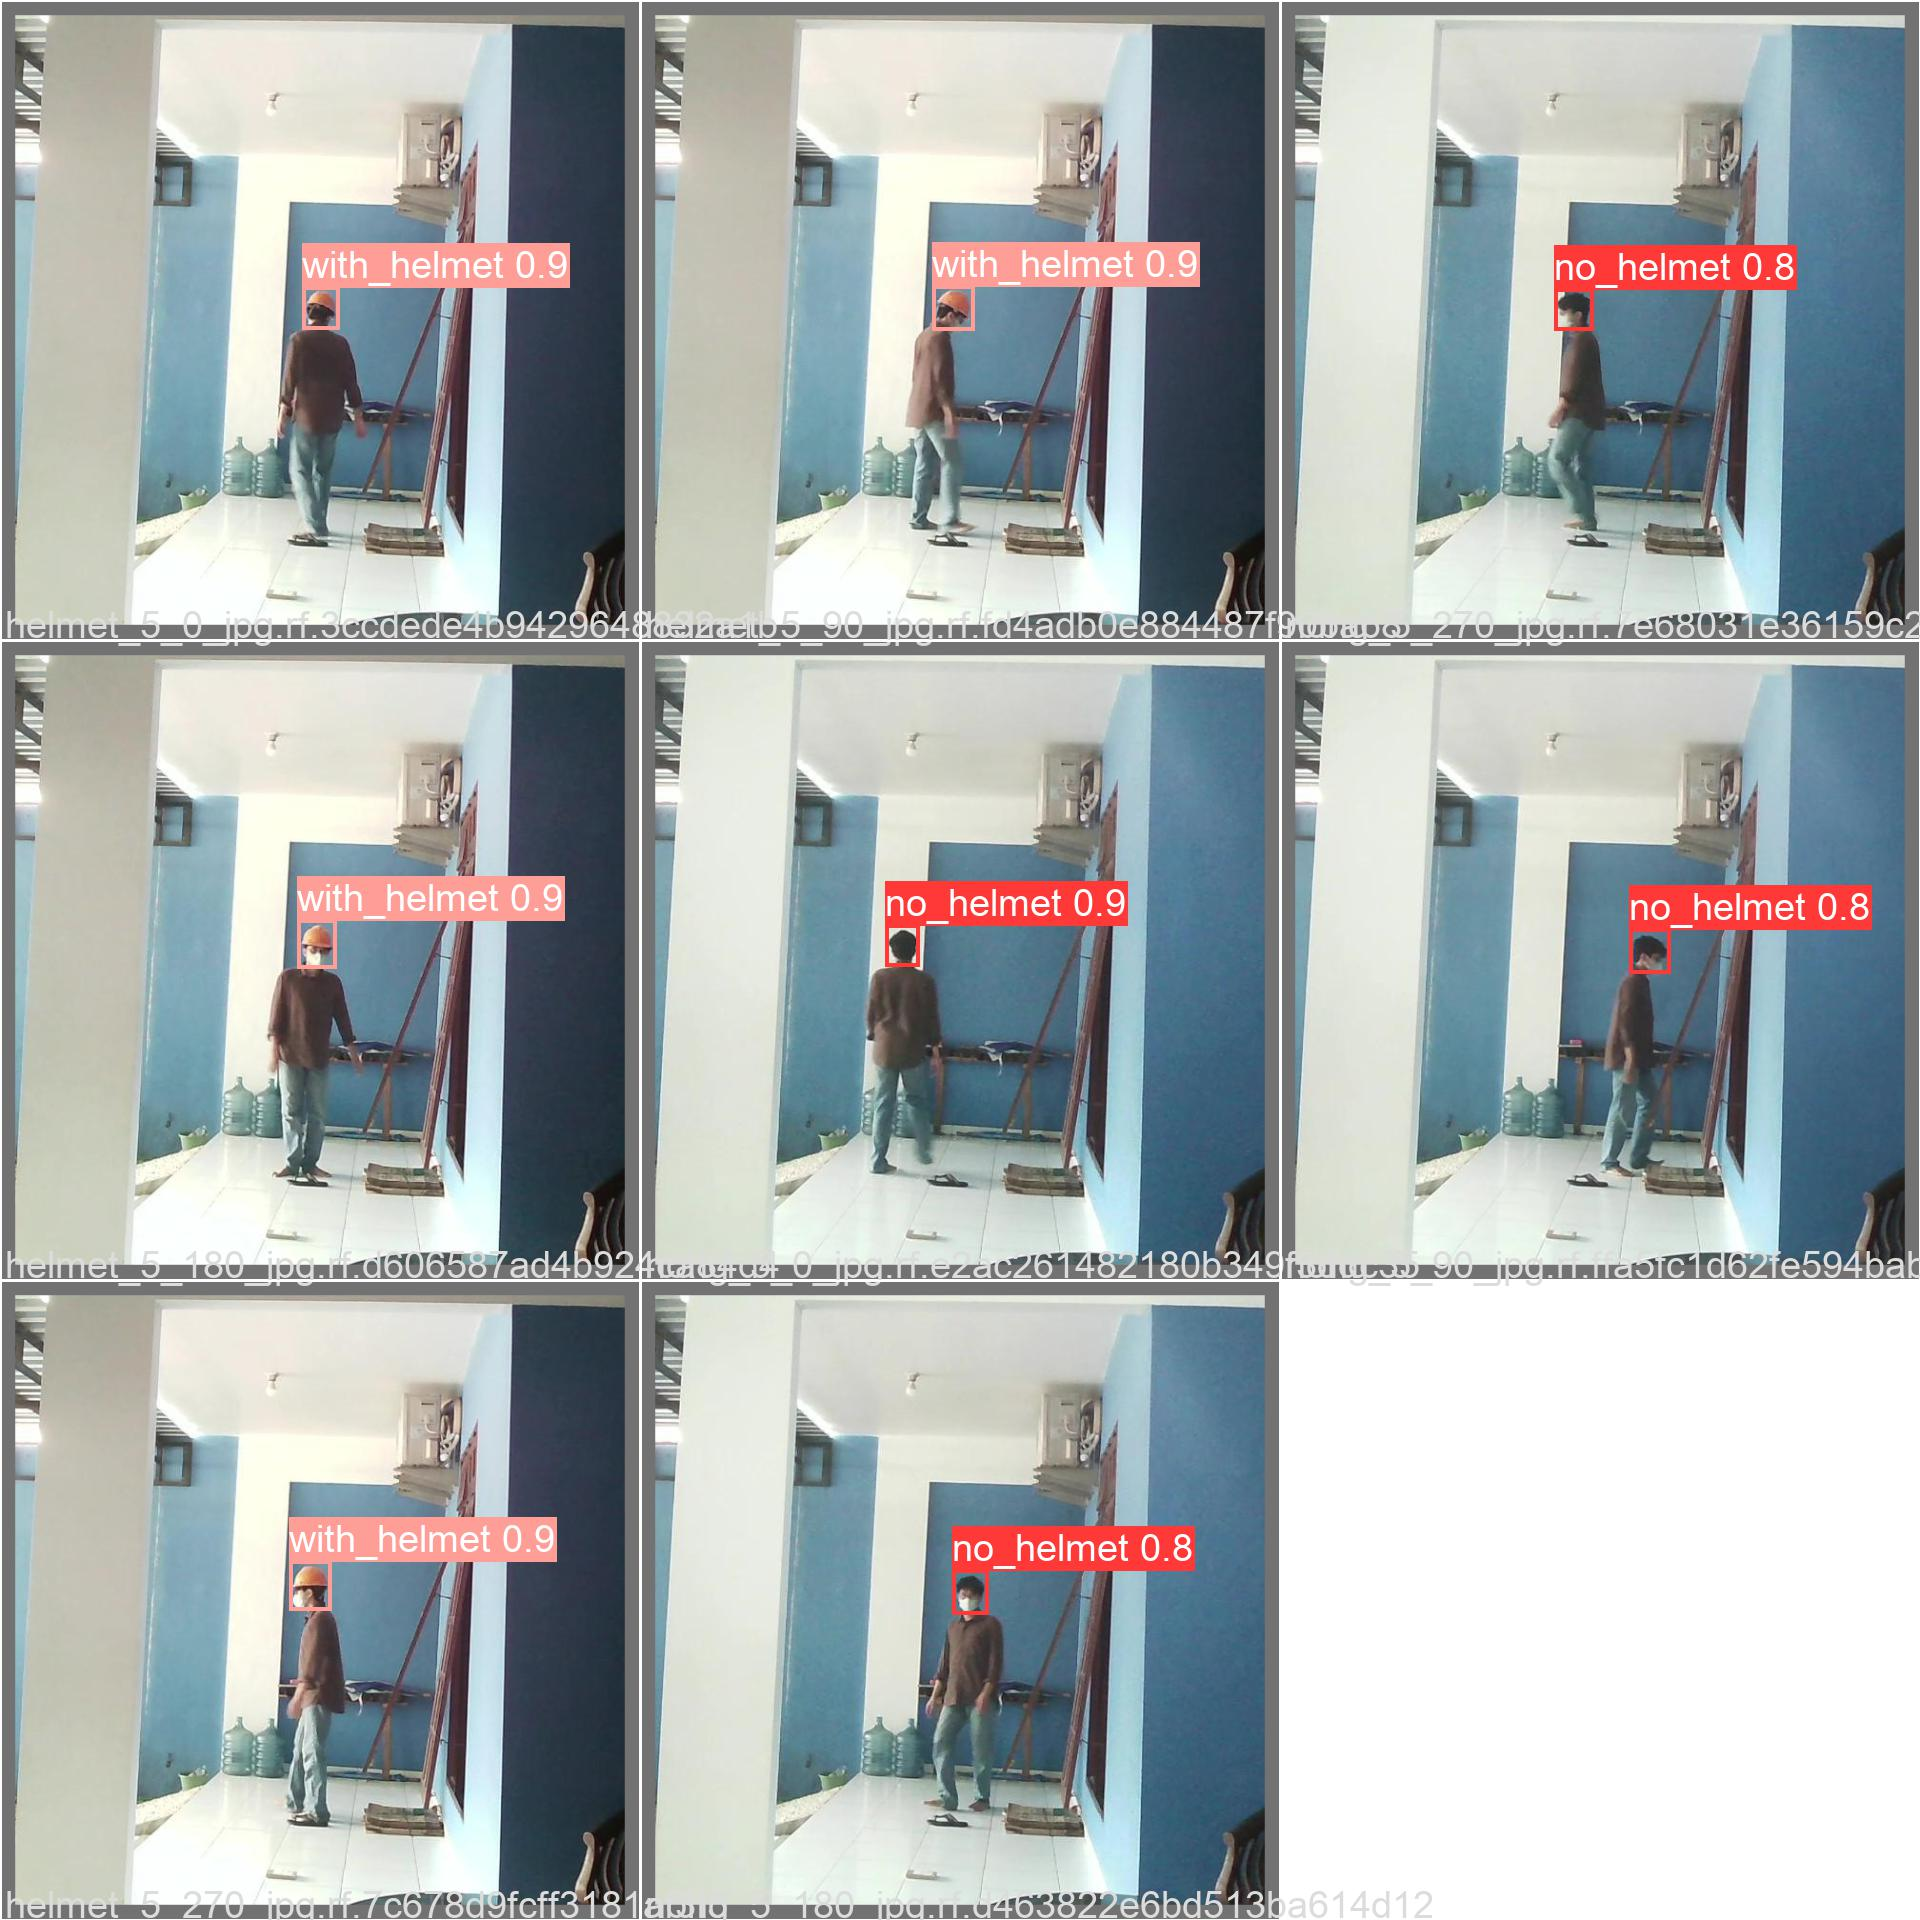
\includegraphics[scale=0.1]{gambar/BerdasarkanJarak/Jarak6_7/val_batch0_pred.jpg}
  \caption{Hasil Prediksi Pada Jarak 6.7 meter}
  % \label{fig:labelbaru}  
\end{figure}

\begin{longtable}{|c|c|c|c|}
  \caption{Konfigurasi Training menggunakan YOLOv5}
  \label{tb:jarak6_7}\\
  \hline
  % \rowcolor[HTML]{C0C0C0}
  \textbf{\emph{Class} }                     & \textbf{\emph{Precision}}  & \textbf{\emph{Recall}} & \textbf{\emph{mAP@.5}}\\
  \hline
  all                                                 & 0.993           & 1        & 0.995         \\
  no\textunderscore helmet                            & 1               & 1        & 0.995          \\
  with\textunderscore helmet                          & 0.986           & 1        & 0.995           \\
  \hline
\end{longtable}


\subsection{Pengujian Pada Jarak 9 Meter}

\begin{figure}[ht]
  \centering
  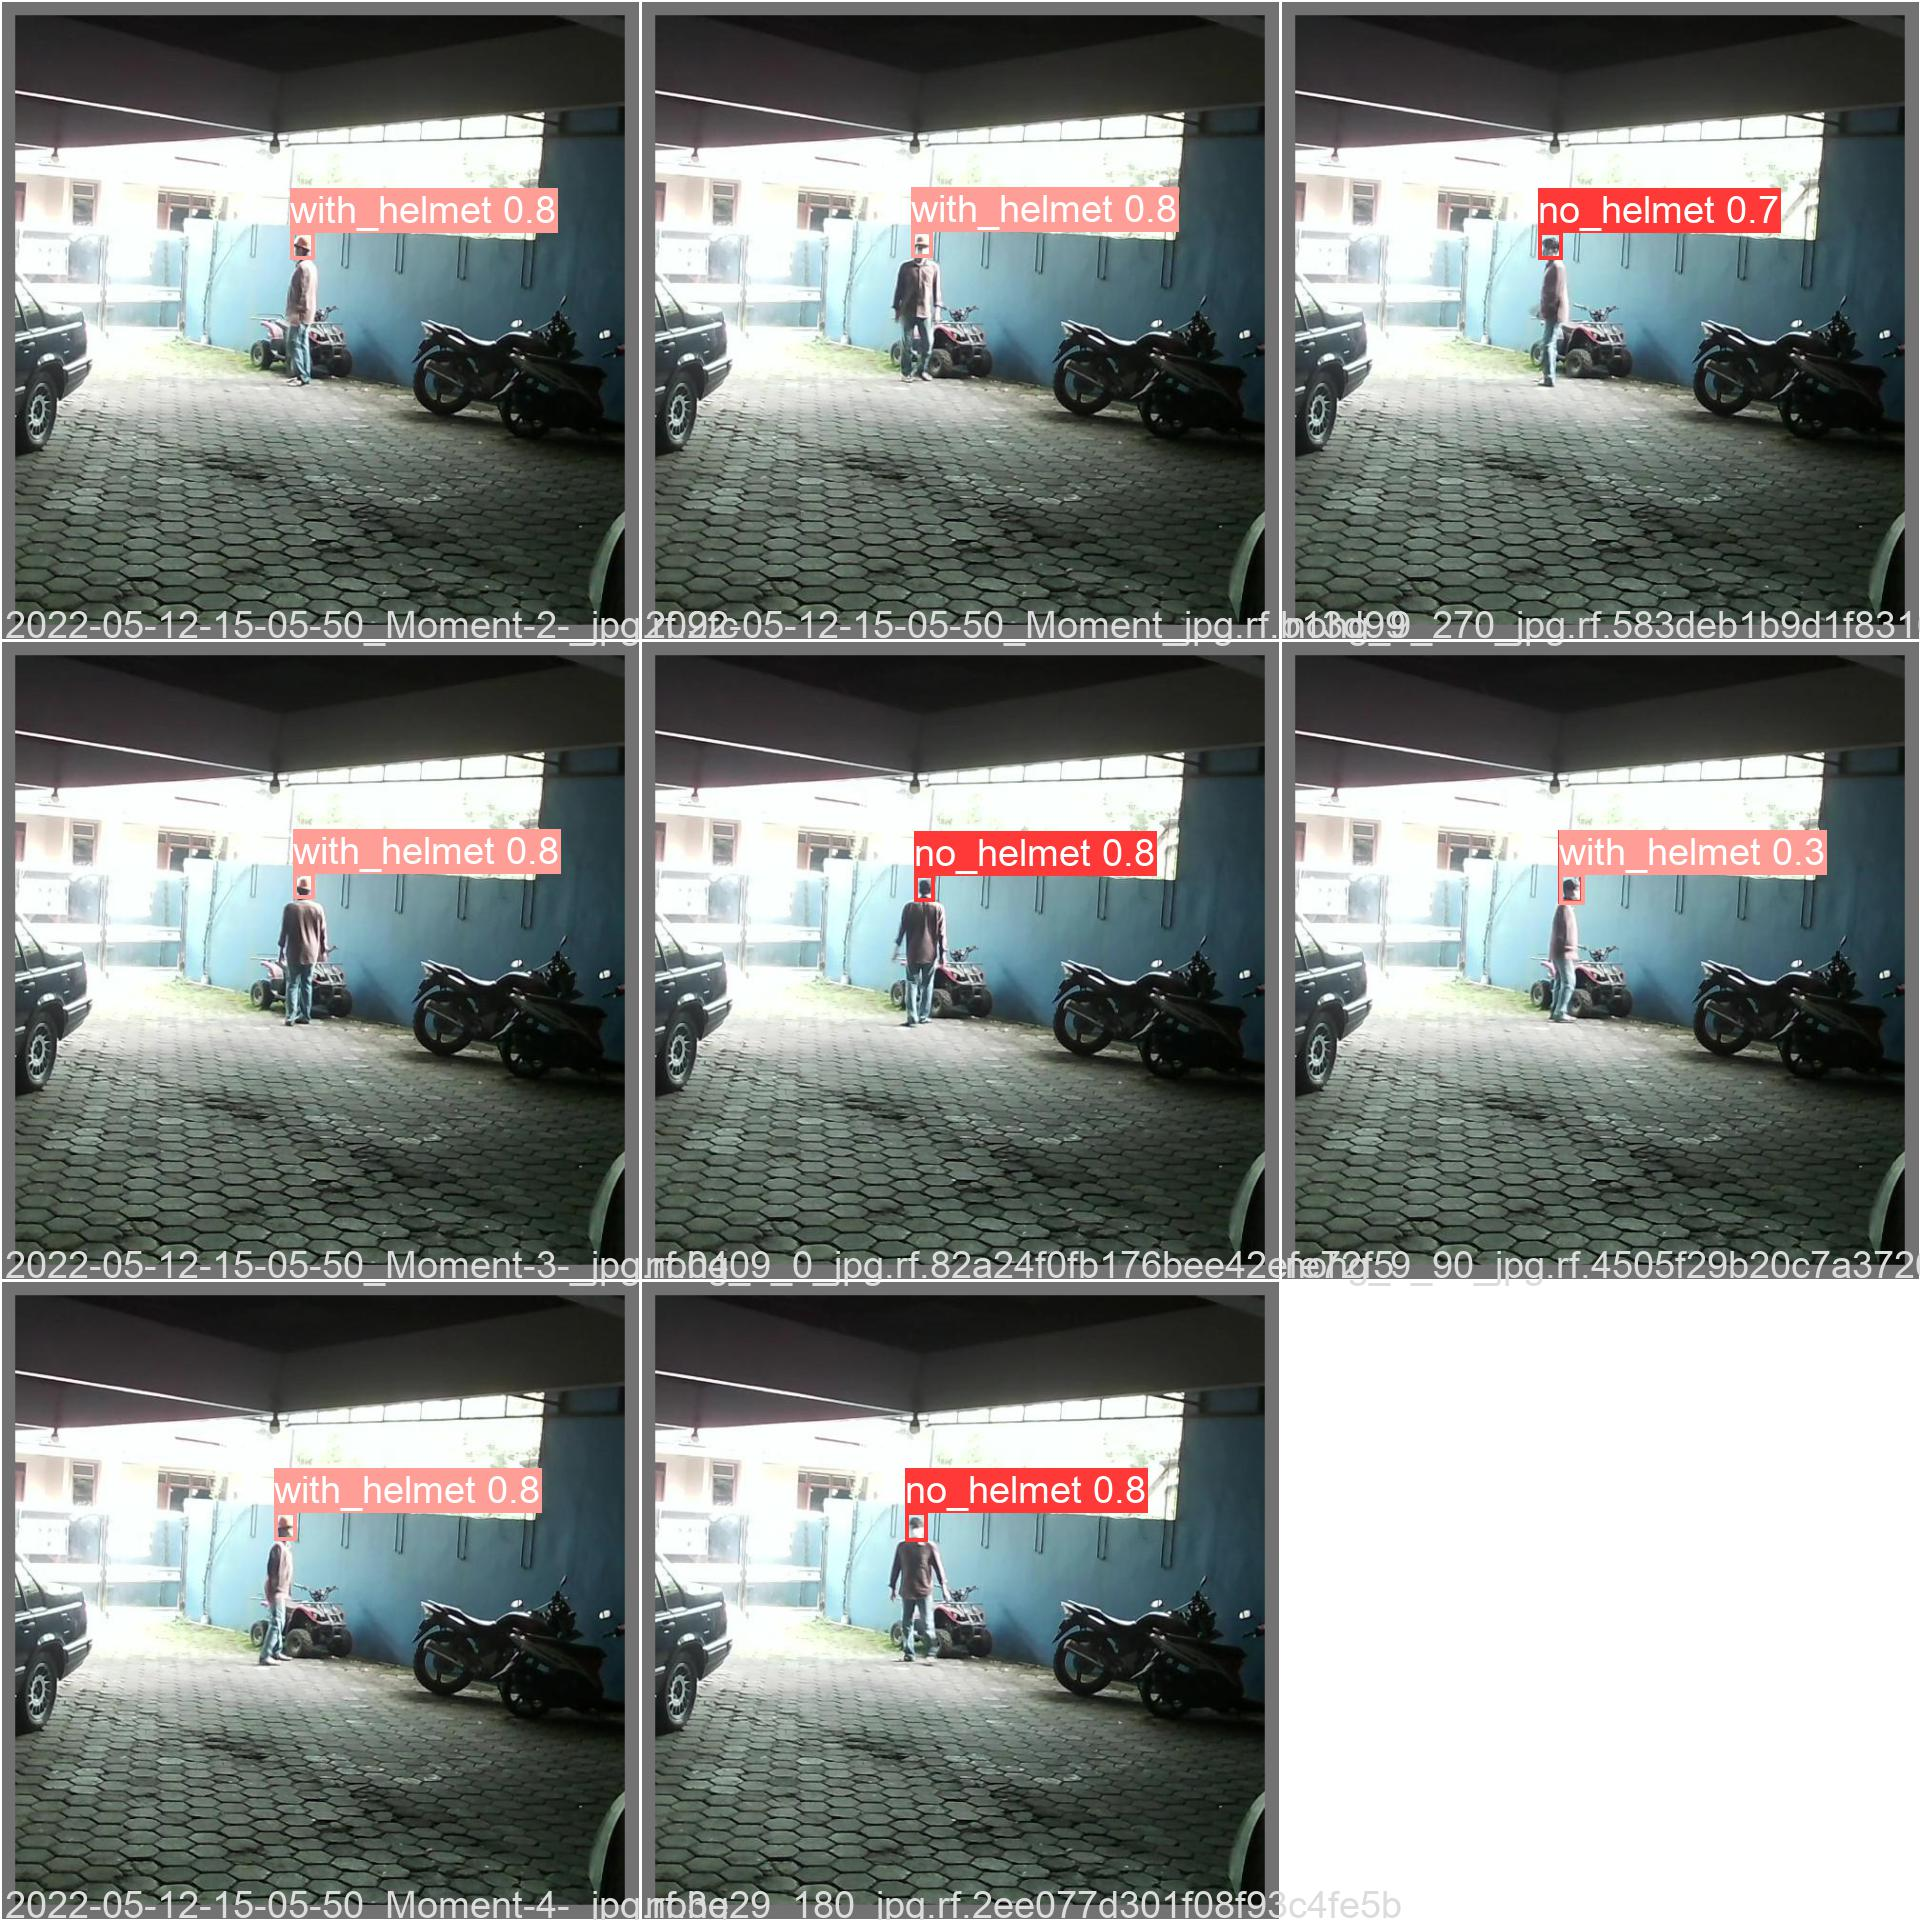
\includegraphics[scale=0.1]{gambar/BerdasarkanJarak/Jarak9/val_batch0_pred.jpg}
  \caption{Hasil Prediksi Pada Jarak 9 meter}
  % \label{fig:labelbaru}  
\end{figure}

\begin{longtable}{|c|c|c|c|}
  \caption{Konfigurasi Training menggunakan YOLOv5}
  \label{tb:jarak9}\\
  \hline
  % \rowcolor[HTML]{C0C0C0}
  \textbf{\emph{Class} }                     & \textbf{\emph{Precision}}  & \textbf{\emph{Recall}} & \textbf{\emph{mAP@.5}}\\
  \hline
  all                                                 & 0.959          & 1        & 0.995         \\
  no\textunderscore helmet                            & 1               & 1        & 0.995          \\
  with\textunderscore helmet                          & 0.918           & 1        & 0.995           \\
  \hline
\end{longtable}